\documentclass{standalone}

\usepackage[T1]{fontenc}
\usepackage[utf8]{inputenc}
\usepackage{eulervm}
\usepackage{amsmath}
\usepackage{bm}
\usepackage{tikz}
\usepackage{environ}
\usepackage{circuitikz}

\usetikzlibrary{fit}
\usetikzlibrary{patterns}
\usetikzlibrary{arrows}
\usetikzlibrary{positioning}

\usepackage{color}

\definecolor{Comment}{RGB}{97,161,176}

\definecolor{btfGreen}{RGB}{51,160,44}
\definecolor{btfRed}{RGB}{190,60,90}

\definecolor{bleuUni}{RGB}{0, 157, 224}
\definecolor{marronUni}{RGB}{68, 58, 49}
\definecolor{grayMarronUni}{RGB}{60, 60, 60}
\definecolor{grayBleuUni}{RGB}{118, 118, 118}

\definecolor{bluecite}{HTML}{009DE0}

\definecolor{Paired-2}{RGB}{166,206,227}
\definecolor{Paired-1}{RGB}{31,120,180}
\definecolor{Paired-4}{RGB}{178,223,138}
\definecolor{Paired-3}{RGB}{51,160,44}
\definecolor{Paired-6}{RGB}{251,154,153}
\definecolor{Paired-5}{RGB}{227,26,28}
\definecolor{Paired-8}{RGB}{253,191,111}
\definecolor{Paired-7}{RGB}{255,127,0}
\definecolor{Paired-10}{RGB}{202,178,214}
\definecolor{Paired-9}{RGB}{106,61,154}
\definecolor{Paired-12}{RGB}{255,255,153}
\definecolor{Paired-11}{RGB}{177,89,40}
\definecolor{Accent-1}{RGB}{127,201,127}
\definecolor{Accent-2}{RGB}{190,174,212}
\definecolor{Accent-3}{RGB}{253,192,134}
\definecolor{Accent-4}{RGB}{255,255,153}
\definecolor{Accent-5}{RGB}{56,108,176}
\definecolor{Accent-6}{RGB}{240,2,127}
\definecolor{Accent-7}{RGB}{191,91,23}
\definecolor{Accent-8}{RGB}{102,102,102}
\definecolor{Spectral-1}{RGB}{158,1,66}
\definecolor{Spectral-2}{RGB}{213,62,79}
\definecolor{Spectral-3}{RGB}{244,109,67}
\definecolor{Spectral-4}{RGB}{253,174,97}
\definecolor{Spectral-5}{RGB}{254,224,139}
\definecolor{Spectral-6}{RGB}{255,255,191}
\definecolor{Spectral-7}{RGB}{230,245,152}
\definecolor{Spectral-8}{RGB}{171,221,164}
\definecolor{Spectral-9}{RGB}{102,194,165}
\definecolor{Spectral-10}{RGB}{50,136,189}
\definecolor{Spectral-11}{RGB}{94,79,162}
\definecolor{Set1-1}{RGB}{228,26,28}
\definecolor{Set1-2}{RGB}{55,126,184}
\definecolor{Set1-3}{RGB}{77,175,74}
\definecolor{Set1-4}{RGB}{152,78,163}
\definecolor{Set1-5}{RGB}{255,127,0}
\definecolor{Set1-6}{RGB}{255,255,51}
\definecolor{Set1-7}{RGB}{166,86,40}
\definecolor{Set1-8}{RGB}{247,129,191}
\definecolor{Set1-9}{RGB}{153,153,153}
\definecolor{Set2-1}{RGB}{102,194,165}
\definecolor{Set2-2}{RGB}{252,141,98}
\definecolor{Set2-3}{RGB}{141,160,203}
\definecolor{Set2-4}{RGB}{231,138,195}
\definecolor{Set2-5}{RGB}{166,216,84}
\definecolor{Set2-6}{RGB}{255,217,47}
\definecolor{Set2-7}{RGB}{229,196,148}
\definecolor{Set2-8}{RGB}{179,179,179}
\definecolor{Dark2-1}{RGB}{27,158,119}
\definecolor{Dark2-2}{RGB}{217,95,2}
\definecolor{Dark2-3}{RGB}{117,112,179}
\definecolor{Dark2-4}{RGB}{231,41,138}
\definecolor{Dark2-5}{RGB}{102,166,30}
\definecolor{Dark2-6}{RGB}{230,171,2}
\definecolor{Dark2-7}{RGB}{166,118,29}
\definecolor{Dark2-8}{RGB}{102,102,102}
\definecolor{Reds-1}{RGB}{255,245,240}
\definecolor{Reds-2}{RGB}{254,224,210}
\definecolor{Reds-3}{RGB}{252,187,161}
\definecolor{Reds-4}{RGB}{252,146,114}
\definecolor{Reds-5}{RGB}{251,106,74}
\definecolor{Reds-6}{RGB}{239,59,44}
\definecolor{Reds-7}{RGB}{203,24,29}
\definecolor{Reds-8}{RGB}{165,15,21}
\definecolor{Reds-9}{RGB}{103,0,13}
\definecolor{Greens-1}{RGB}{247,252,245}
\definecolor{Greens-2}{RGB}{229,245,224}
\definecolor{Greens-3}{RGB}{199,233,192}
\definecolor{Greens-4}{RGB}{161,217,155}
\definecolor{Greens-5}{RGB}{116,196,118}
\definecolor{Greens-6}{RGB}{65,171,93}
\definecolor{Greens-7}{RGB}{35,139,69}
\definecolor{Greens-8}{RGB}{0,109,44}
\definecolor{Greens-9}{RGB}{0,68,27}
\definecolor{Blues-1}{RGB}{247,251,255}
\definecolor{Blues-2}{RGB}{222,235,247}
\definecolor{Blues-3}{RGB}{198,219,239}
\definecolor{Blues-4}{RGB}{158,202,225}
\definecolor{Blues-5}{RGB}{107,174,214}
\definecolor{Blues-6}{RGB}{66,146,198}
\definecolor{Blues-7}{RGB}{33,113,181}
\definecolor{Blues-8}{RGB}{8,81,156}
\definecolor{Blues-9}{RGB}{8,48,107}


\begin{document}
  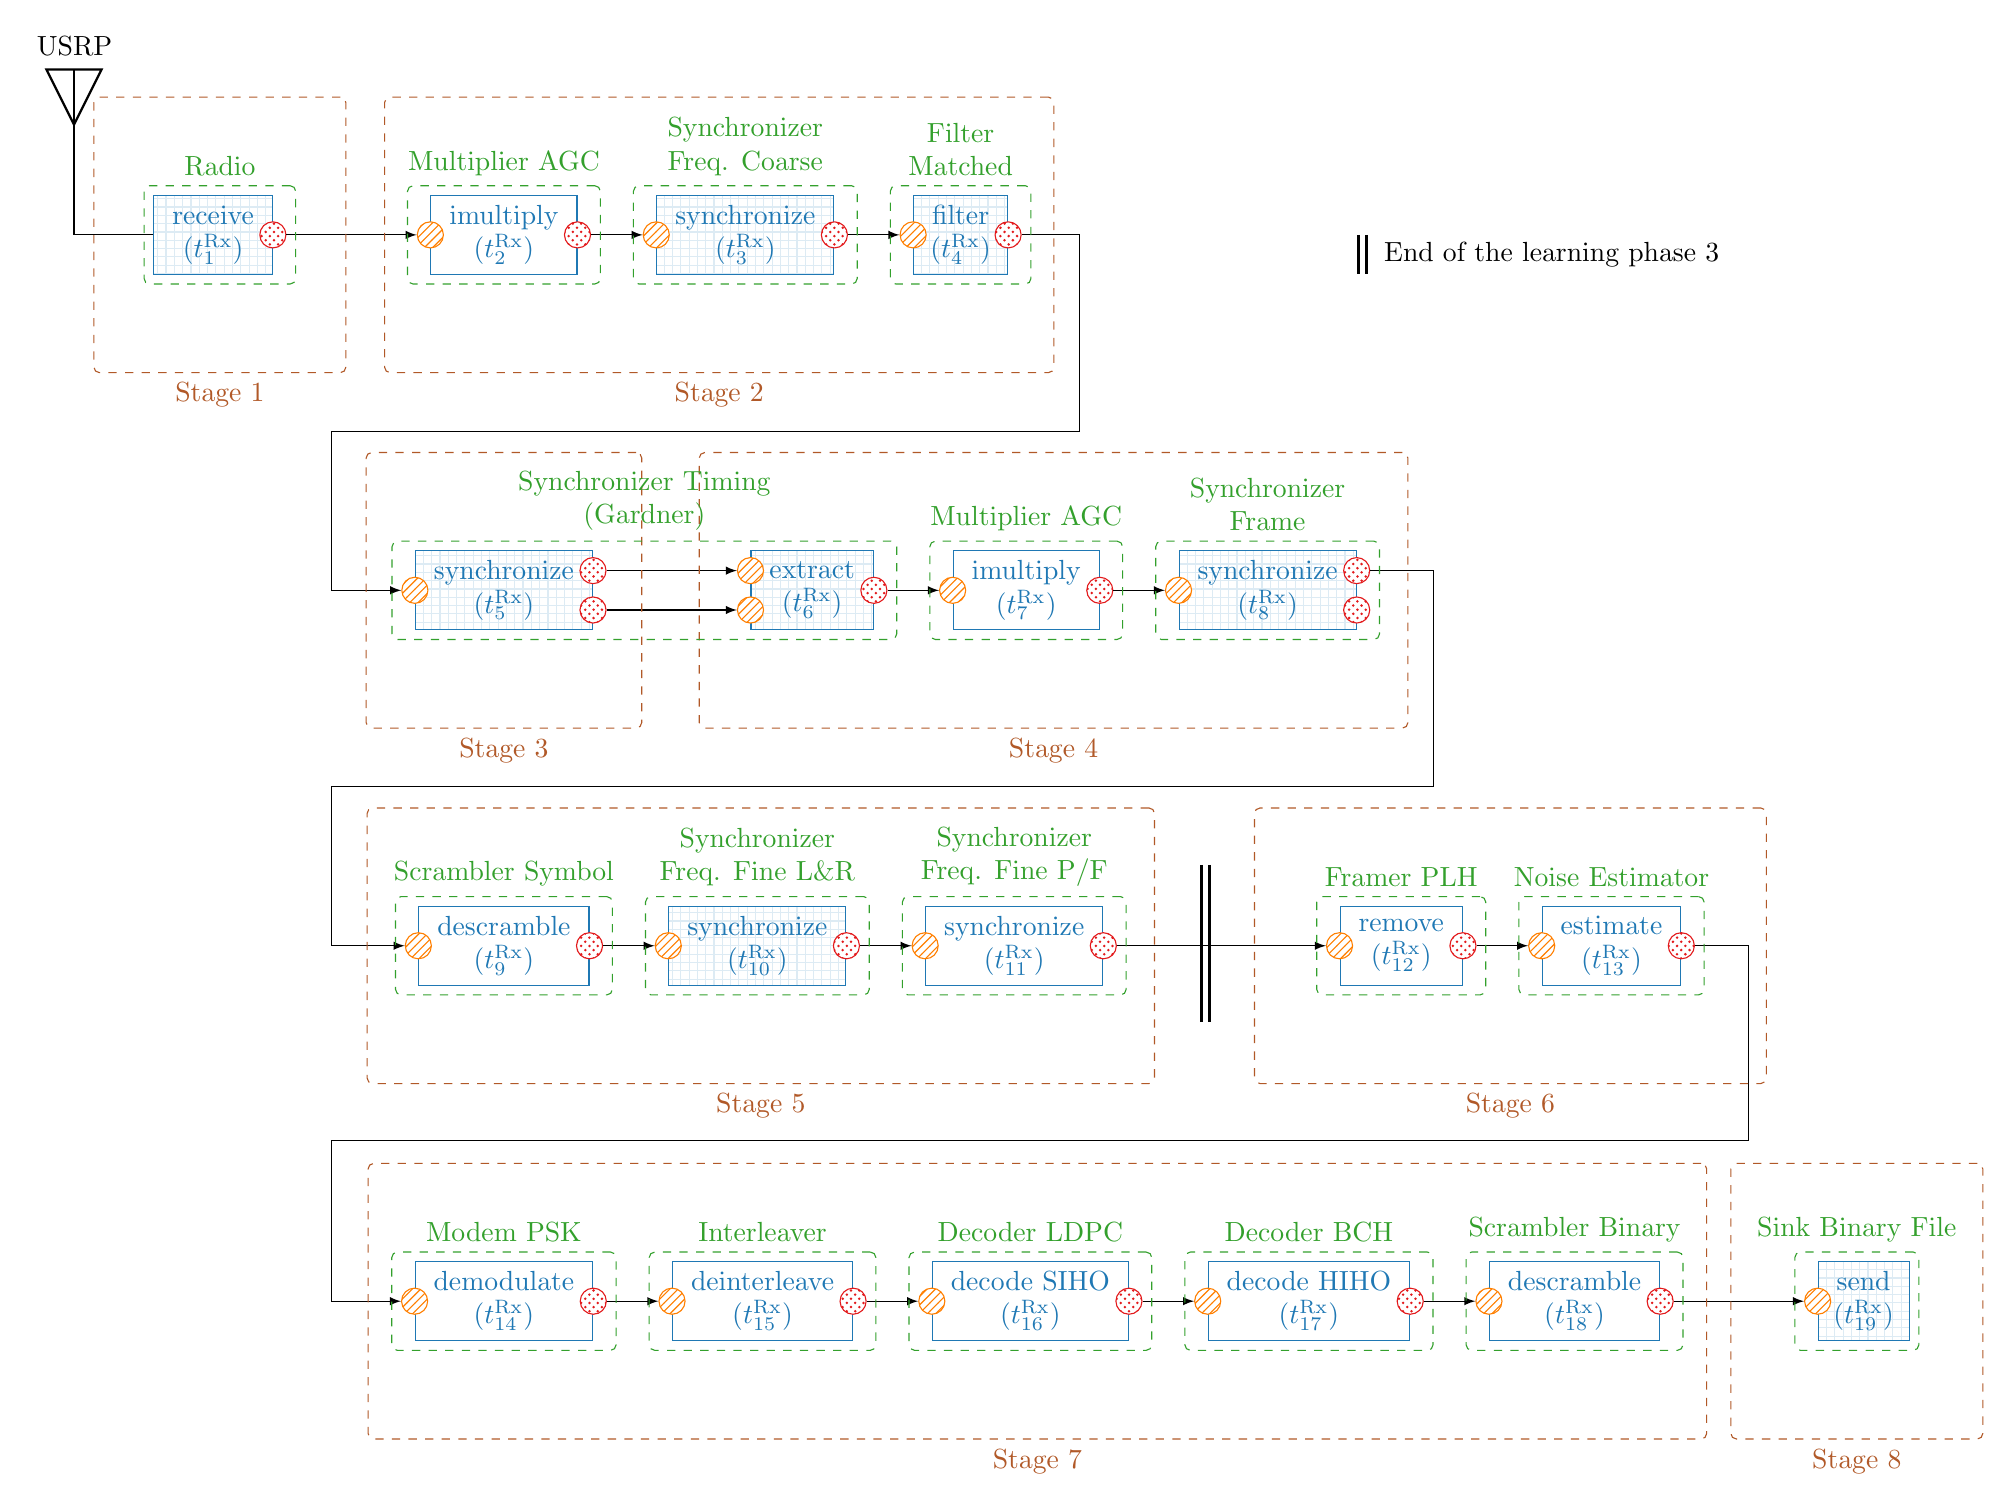
\begin{tikzpicture}%[scale=\tikzscale]
    \tikzset{ tsk/.style ={draw=Paired-1, rounded corners=0pt, text=Paired-1, minimum height=1.0cm, minimum width=1cm} }
    \tikzset{ stsk/.style={draw=Paired-1, rounded corners=0pt, text=Paired-1, minimum height=1.0cm, minimum width=1cm, preaction={fill=white}, pattern=grid, pattern color=Paired-1!15} }
    \tikzset{ ss/.style  ={draw=Paired-9, rounded corners=2pt, minimum height=1.5cm} }
    \tikzset{ seq/.style ={draw=Paired-11, dashed, rounded corners=2pt} }
    \tikzset{ mdl/.style ={draw=Paired-3,  dashed, rounded corners=2pt} }
    \tikzset{ pip/.style ={draw=Dark2-8,  dotted, thick, rounded corners=2pt} }
    \tikzset{ sin/.style ={draw=Paired-7, circle, minimum width=0.3cm, text=black, preaction={fill=white}, pattern=north east lines, pattern color=Paired-7} }
    \tikzset{ sout/.style={draw=Paired-5, circle, minimum width=0.3cm, text=black, preaction={fill=white}, pattern=crosshatch dots, pattern color=Paired-5} }

    \node[stsk                     , align=center] (t1) at ( 0.0, 2.0) {~receive~~\\($t^{\text{Rx}}_1$)};
    \node[tsk , right=2.00cm of t1 , align=center] (t2)                {~imultiply~~\\($t^{\text{Rx}}_2$)};
    \node[stsk, right=1.00cm of t2 , align=center] (t3)                {~synchronize~~\\($t^{\text{Rx}}_3$)};
    \node[stsk, right=1.00cm of t3 , align=center] (t4)                {~filter~~\\($t^{\text{Rx}}_4$)};
    \node[stsk, below=3.50cm of t2 , align=center] (t5)                {~synchronize~~\\($t^{\text{Rx}}_5$)};
    \node[stsk, right=2.00cm of t5 , align=center] (t6)                {~extract~~\\($t^{\text{Rx}}_6$)};
    \node[tsk , right=1.00cm of t6 , align=center] (t7)                {~imultiply~~\\($t^{\text{Rx}}_7$)};
    \node[stsk, right=1.00cm of t7 , align=center] (t8)                {~synchronize~~\\($t^{\text{Rx}}_8$)};
    \node[tsk , below=3.50cm of t5 , align=center] (t9)                {~descramble~~\\($t^{\text{Rx}}_9$)};
    \node[stsk, right=1.00cm of t9 , align=center] (t10)               {~synchronize~~\\($t^{\text{Rx}}_{10}$)};
    \node[tsk , right=1.00cm of t10, align=center] (t11)               {~synchronize~~\\($t^{\text{Rx}}_{11}$)};
    \node[tsk , right=3.00cm of t11, align=center] (t12)               {~remove~~\\($t^{\text{Rx}}_{12}$)};
    \node[tsk , right=1.00cm of t12, align=center] (t13)               {~estimate~~\\($t^{\text{Rx}}_{13}$)};
    \node[tsk , below=3.50cm of t9 , align=center] (t14)               {~demodulate~~\\($t^{\text{Rx}}_{14}$)};
    \node[tsk , right=1.00cm of t14, align=center] (t15)               {~deinterleave~~\\($t^{\text{Rx}}_{15}$)};
    \node[tsk , right=1.00cm of t15, align=center] (t16)               {~decode SIHO~~\\($t^{\text{Rx}}_{16}$)};
    \node[tsk , right=1.00cm of t16, align=center] (t17)               {~decode HIHO~~\\($t^{\text{Rx}}_{17}$)};
    \node[tsk , right=1.00cm of t17, align=center] (t18)               {~descramble~~\\($t^{\text{Rx}}_{18}$)};
    \node[stsk, right=2.00cm of t18, align=center] (t19)               {~send~~\\($t^{\text{Rx}}_{19}$)};

    \node[sout, at=(t1.east)                ] (t1_so)  {};
    \node[sin,  at=(t2.west)                ] (t2_si)  {};
    \node[sout, at=(t2.east)                ] (t2_so)  {};
    \node[sin,  at=(t3.west)                ] (t3_si)  {};
    \node[sout, at=(t3.east)                ] (t3_so)  {};
    \node[sin,  at=(t4.west)                ] (t4_si)  {};
    \node[sout, at=(t4.east)                ] (t4_so)  {};
    \node[sin,  at=(t5.west)                ] (t5_si)  {};
    \node[sout, at=(t5.east), yshift=+0.25cm] (t5_so1) {};
    \node[sout, at=(t5.east), yshift=-0.25cm] (t5_so2) {};
    \node[sin,  at=(t6.west), yshift=+0.25cm] (t6_si1) {};
    \node[sin,  at=(t6.west), yshift=-0.25cm] (t6_si2) {};
    \node[sout, at=(t6.east)                ] (t6_so)  {};
    \node[sin,  at=(t7.west)                ] (t7_si)  {};
    \node[sout, at=(t7.east)                ] (t7_so)  {};
    \node[sin,  at=(t8.west)                ] (t8_si)  {};
    \node[sout, at=(t8.east), yshift=+0.25cm] (t8_so1) {};
    \node[sout, at=(t8.east), yshift=-0.25cm] (t8_so2) {};
    \node[sin,  at=(t9.west)                ] (t9_si)  {};
    \node[sout, at=(t9.east)                ] (t9_so)  {};
    \node[sin,  at=(t10.west)               ] (t10_si) {};
    \node[sout, at=(t10.east)               ] (t10_so) {};
    \node[sin,  at=(t11.west)               ] (t11_si) {};
    \node[sout, at=(t11.east)               ] (t11_so) {};
    \node[sin,  at=(t12.west)               ] (t12_si) {};
    \node[sout, at=(t12.east)               ] (t12_so) {};
    \node[sin,  at=(t13.west)               ] (t13_si) {};
    \node[sout, at=(t13.east)               ] (t13_so) {};
    \node[sin,  at=(t14.west)               ] (t14_si) {};
    \node[sout, at=(t14.east)               ] (t14_so) {};
    \node[sin,  at=(t15.west)               ] (t15_si) {};
    \node[sout, at=(t15.east)               ] (t15_so) {};
    \node[sin,  at=(t16.west)               ] (t16_si) {};
    \node[sout, at=(t16.east)               ] (t16_so) {};
    \node[sin,  at=(t17.west)               ] (t17_si) {};
    \node[sout, at=(t17.east)               ] (t17_so) {};
    \node[sin,  at=(t18.west)               ] (t18_si) {};
    \node[sout, at=(t18.east)               ] (t18_so) {};
    \node[sin,  at=(t19.west)               ] (t19_si) {};

    \draw[black, -] (t1.west)--++(0:-1.0cm) node[antenna, label={[above,yshift=+2.15cm]USRP}] {};
    \draw[->,>=latex] (t1_so) -- (t2_si)  node [midway, above] {};
    \draw[->,>=latex] (t2_so) -- (t3_si)  node [midway, above] {};
    \draw[->,>=latex] (t3_so) -- (t4_si)  node [midway, above] {};
    % \draw[->,>=latex] (t4_so) -- (t5_si)  node [midway, above] {};
    \draw[->,>=latex] (t4_so) -| (11.0,-0.5) -- (1.5,-0.5) |- (t5_si)  node [midway, above] {};
    \draw[->,>=latex] (t5_so1) -- (t6_si1)  node [midway, above] {};
    \draw[->,>=latex] (t5_so2) -- (t6_si2)  node [midway, above] {};
    % \draw[->,>=latex] (t5_so) -- (13.9,2.0) -- (13.9,1.15) -- (2.25,1.15) -- (2.25,0) -- (t6_si)  node [midway, above] {};
    \draw[->,>=latex] (t6_so) -- (t7_si)  node [midway, above] {};
    \draw[->,>=latex] (t7_so) -- (t8_si)  node [midway, above] {};
    % \draw[->,>=latex] (t8_so) -- (t9_si)  node [midway, above] {};
    \draw[->,>=latex] (t8_so1) -| (15.5,-5.0) -- (1.5,-5.0) |- (t9_si)  node [midway, above] {};
    \draw[->,>=latex] (t9_so) -- (t10_si) node [midway, above] {};
    \draw[->,>=latex] (t10_so) -- (t11_si) node [midway, above] {};
    \draw[->,>=latex] (t11_so) -- (t12_si) node [midway, above] {};
    \draw[->,>=latex] (t12_so) -- (t13_si) node [midway, above] {};
    % \draw[->,>=latex] (t13_so) -- (t14_si) node [midway, above] {};
    \draw[->,>=latex] (t13_so) -| (19.5,-9.5) -- (1.5,-9.5) |- (t14_si)  node [midway, above] {};

    \draw[->,>=latex] (t14_so) -- (t15_si) node [midway, above] {};
    \draw[->,>=latex] (t15_so) -- (t16_si) node [midway, above] {};
    \draw[->,>=latex] (t16_so) -- (t17_si) node [midway, above] {};
    \draw[->,>=latex] (t17_so) -- (t18_si) node [midway, above] {};
    \draw[->,>=latex] (t18_so) -- (t19_si) node [midway, above] {};

    \node[seq, minimum height=3.5cm, minimum width=3.2cm,   label={[Paired-11]below:Stage 1}, fit=(t1)  (t1_so)                                                          ] (seq1) {};
    \node[seq, minimum height=3.5cm, minimum width=8.5cm,   label={[Paired-11]below:Stage 2}, fit=(t2)  (t2_si)  (t2_so)  (t3)  (t3_si)  (t3_so)  (t4)  (t4_si)  (t4_so) ] (seq2) {};
    \node[seq, minimum height=3.5cm, minimum width=3.5cm,   label={[Paired-11]below:Stage 3}, fit=(t5)  (t5_si)  (t5_so1)                                                ] (seq3) {};
    \node[seq, minimum height=3.5cm, minimum width=9.0cm,   label={[Paired-11]below:Stage 4}, fit=(t6)  (t6_si1) (t6_so)  (t7)  (t7_si)  (t7_so)  (t8)  (t8_si)  (t8_so1)] (seq4) {};
    \node[seq, minimum height=3.5cm, minimum width=10.0cm,  label={[Paired-11]below:Stage 5}, fit=(t9)  (t9_si)  (t9_so)  (t10) (t10_si) (t10_so) (t11) (t11_si) (t11_so)] (seq5) {};
    \node[seq, minimum height=3.5cm, minimum width=6.5cm,   label={[Paired-11]below:Stage 6}, fit=(t12) (t12_si) (t12_so) (t13) (t13_si) (t13_so)                        ] (seq6) {};
    \node[seq, minimum height=3.5cm, minimum width=17.0cm,  label={[Paired-11]below:Stage 7}, fit=(t14_si) (t18_so)                                                      ] (seq7) {};
    \node[seq, minimum height=3.5cm, minimum width=3.2cm,   label={[Paired-11]below:Stage 8}, fit=(t19_si) (t19)                                                         ] (seq8) {};

    \node[mdl, label={[Paired-3, align=center]above:Radio},                          fit=(t1)           (t1_so)     ] (m1)  {};
    \node[mdl, label={[Paired-3, align=center]above:Multiplier AGC},                 fit=(t2)  (t2_si)  (t2_so)     ] (m2)  {};
    \node[mdl, label={[Paired-3, align=center]above:Synchronizer\\Freq. Coarse},     fit=(t3)  (t3_si)  (t3_so)     ] (m3)  {};
    \node[mdl, label={[Paired-3, align=center]above:Filter\\Matched},                fit=(t4)  (t4_si)  (t4_so)     ] (m4)  {};
    \node[mdl, label={[Paired-3, align=center]above:Synchronizer Timing\\(Gardner)}, fit=(t5)  (t5_si)  (t6) (t6_so)] (m5)  {};
    \node[mdl, label={[Paired-3, align=center]above:Multiplier AGC},                 fit=(t7)  (t7_si)  (t7_so)     ] (m6)  {};
    \node[mdl, label={[Paired-3, align=center]above:Synchronizer\\Frame},            fit=(t8)  (t8_si)  (t8_so1)    ] (m7)  {};
    \node[mdl, label={[Paired-3, align=center]above:Scrambler Symbol},               fit=(t9)  (t9_si)  (t9_so)     ] (m8)  {};
    \node[mdl, label={[Paired-3, align=center]above:Synchronizer\\Freq. Fine L\&R},  fit=(t10) (t10_si) (t10_so)    ] (m9)  {};
    \node[mdl, label={[Paired-3, align=center]above:Synchronizer\\Freq. Fine P/F},   fit=(t11) (t11_si) (t11_so)    ] (m10) {};
    \node[mdl, label={[Paired-3, align=center]above:Framer PLH},                     fit=(t12) (t12_si) (t12_so)    ] (m11) {};
    \node[mdl, label={[Paired-3, align=center]above:Noise Estimator},                fit=(t13) (t13_si) (t13_so)    ] (m12) {};
    \node[mdl, label={[Paired-3, align=center]above:Modem PSK},                      fit=(t14) (t14_si) (t14_so)    ] (m13) {};
    \node[mdl, label={[Paired-3, align=center]above:Interleaver},                    fit=(t15) (t15_si) (t15_so)    ] (m14) {};
    \node[mdl, label={[Paired-3, align=center]above:Decoder LDPC},                   fit=(t16) (t16_si) (t16_so)    ] (m15) {};
    \node[mdl, label={[Paired-3, align=center]above:Decoder BCH},                    fit=(t17) (t17_si) (t17_so)    ] (m16) {};
    \node[mdl, label={[Paired-3, align=center]above:Scrambler Binary},               fit=(t18) (t18_si) (t18_so)    ] (m17) {};
    \node[mdl, label={[Paired-3, align=center]above:Sink Binary File},               fit=(t19) (t19_si)             ] (m18) {};


    \draw[-,>=latex, very thick] (12.55,-6.0) -- (12.55,-8) node [midway, above] {};
    \draw[-,>=latex, very thick] (12.65,-6.0) -- (12.65,-8) node [midway, above] {};
    \draw[-,>=latex, very thick] (14.55,2.0) -- (14.55,1.5) node [midway, above] {};
    \draw[-,>=latex, very thick] (14.65,2.0) -- (14.65,1.5) node [midway, above] {};
    \node at (17.00,1.75) {End of the learning phase 3};
  \end{tikzpicture}
\end{document}